\section{The Kandinsky Model}
\subsection{Introduction}
\subsection{Area Investigation}
The idea of the stretching technique is to create new space between edges and vertices. By doing so, the space for circular arcs will be guaranteed. As we already saw, the stretching technique is sufficient for 4-planar graph drawings. But what about planar drawings of arbitrary degree?\\
There are two major cases to distinguish - either a vertical line segment is between two other segments or it is connected to a vertex therefore on one of the ends of the polyedge.
\subsubsection{Between two segments - \grqq Boxing\grqq}
The stretching technique is a modification of an input graph fulfilling properties of the Fixed Shape Model. In this section we will examine the resulting space along vertical line segments. We will see that the new space created can be described as squares or \grqq boxes\grqq.
We will see that the stretching technique will result in new space left and right from it.
\begin{lemma}
	Let $l$ be the longest vertical line segment in a given orthogonal drawing of a graph $G$. Then, after applying the stretching technique by the factor of $|l|$, every vertical line segment $l'$ which is between two segments got a new box of space left and right from it of size $l'\times l \leq (l')^2$.\label{lem:space_stretch}
\end{lemma}
\begin{proof}
	Let $l'$ be a vertical line segment between two horizontal line segments. Then, by planarity of the orthogonal drawing, consider without loss of generality the minimum distance between $l'$ and another vertical line segment $l''$ by $\delta(l',l'') \geq 1$ on the fine integer grid. Stretching every horizontal line segment by adding a segment of size $|l|$ results in a stretching of the distance of two vertical line segments. The distance of vertical line segments can be considered as a horizontal substraction. $$\delta(l',l'') = |l'_x - l''_x|$$
Stretching horizontally modifies the position of objects in x-coordinates only.
\begin{align}
\delta'(l',l'') = &|\left(|l| + |l'_x|) - (|l| + |l''_x|\right)|\\
 \underbrace{=}_{|l| > 0} &|l| + \left(|l'_x - l''_x|\right) = |l| + \delta(l',l'')
\end{align}
So the distance between a vertical line and an object increased to minimum $|l|+1$.
\end{proof}
\begin{figure}[h]
	\centering
	\begin{subfigure}{0.3\textwidth}
			\centering
			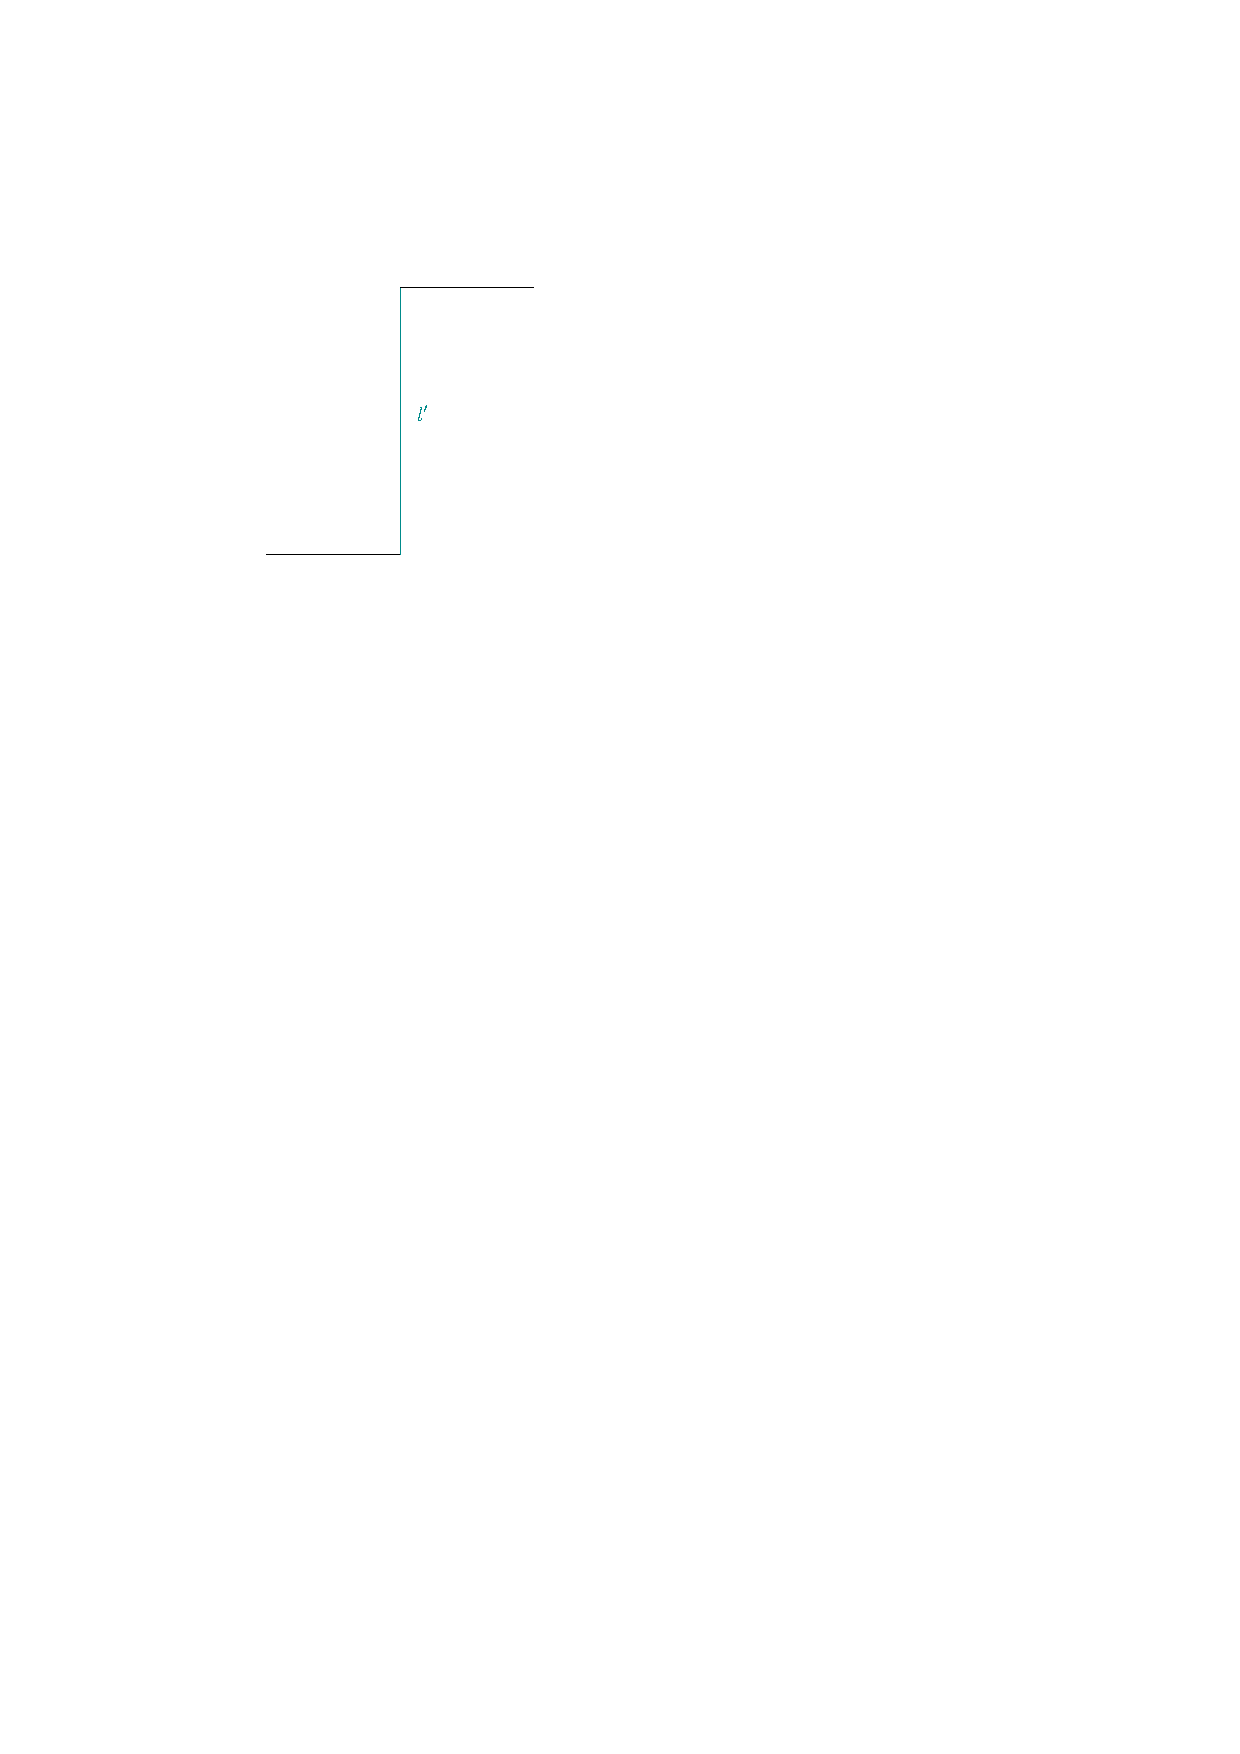
\includegraphics[width=0.7\linewidth,page=1]{includegraphics/boxing_alt.pdf}
			\caption{Orthogonal input edge}
	\end{subfigure}
	\begin{subfigure}{0.66\textwidth}
			\centering
			\includegraphics[width=0.7\linewidth,page=2]{includegraphics/boxing_alt.pdf}
			\caption{Two circular arcs result in +1 bend}
\end{subfigure}
	\caption{The $l'\times l'$ box left and right from the original vertical line is empty after applying the stretching technique}
\end{figure}
This implies that there is new space to the left and right of a vertical line $l'$ between two segments of size $|l'|\times|l'|$. We will consider the new space as a free \grqq box\grqq. This means that the space for different situations of SMOG substitution is guaranteed in the intermediate case.
\begin{lemma}
Let $l'$ be the vertical line intermediate in a uniform fragment. Then, take the box of the corresponding side and draw a half circle segment with radius $r = \frac{l'}{2}$. Furthermore, the complexity does not increase.
\end{lemma}
\begin{proof}
	Let $l'$ be the vertical line intermediate in an alternating fragment. Then, take the box of size $|l'| \times |l'|$ and center it around $l'$. Draw two quarter circle segment with the same radii $r = \frac{l'}{2}$ along the alternation. The space is already guaranteed, all left to demonstrate is the complexity increase which takes two bends away (get rid of the vertical line) and substitute with two quarter circle segments which result in three new bends.
\end{proof}
\subsubsection{Connected to a vertex}
If a vertical segment is connected to a vertex, then the boxing argument does not apply, since the space between multiple ports on the same side of a vertex is not altered by the stretching technique. We will see that this will not lead to a problem.
\begin{definition}
	The \textit{bend of end} property of an orthogonal drawing of a graph means that from every polyedge connected to a specific port of a vertex at most one is connected to another vertex with an edge complexity of one. The remaining polyedges are at least of complexity two and bend in some point.
\end{definition}
\begin{lemma}
	Let $\Gamma_G$ be any orthogonal Kandinsky drawing and $v \in V_G$ a vertex with its ports. Then, there is at most one edge connected to each port of $v$ with only one edge segment (complexity = 1). This describes the \textit{bend or end} property of the polyedges regarding a single port.\label{lem:bend_or_end}
\end{lemma}
\begin{proof}
	The vertices inherit a uniform size and are centered on a grid point. Either, a vertex is connected to another vertex with a single segment. Then, the center of both vertices share either the same $x$ or the $y$ coordinate. If two vertices are connected with a polyedge, then it has to bend at some point. The bend or end property of Kandinsky graphs is implied by the coarse grid on which the vertices are positioned. 
\end{proof}
So, regarding a port of a vertex $v$, the edges either bend or end in a vertex. Now we want to examine the space regarding the circular arcs of the SMOG model.
\begin{lemma}
	Consider a vertex $v$ and $p$ edges connected to a port. Then, in SMOG, at most one of the $p$ edges consists of a single segment ending in a vertex (as in Kandinsky). The other minimal $p-1$ edges start off with a circular arc, the original bend wanders along the horizontal segment and - most importantly - the complexity does not increase.\label{lem:Kandinsky_bend}
\end{lemma}
\begin{proof}
	The edge consisting of a single segment is not altered if it is vertical. If it is horizonal, the stretching technique adds the length of the longest segment. Therefore it does not change in its characteristics, only in length.\\
	Consider the other minimal $p-1$ edges which are bending in some point.\\
	\begin{figure}[h]
		\centering
		\begin{subfigure}{0.3\textwidth}
			\centering
			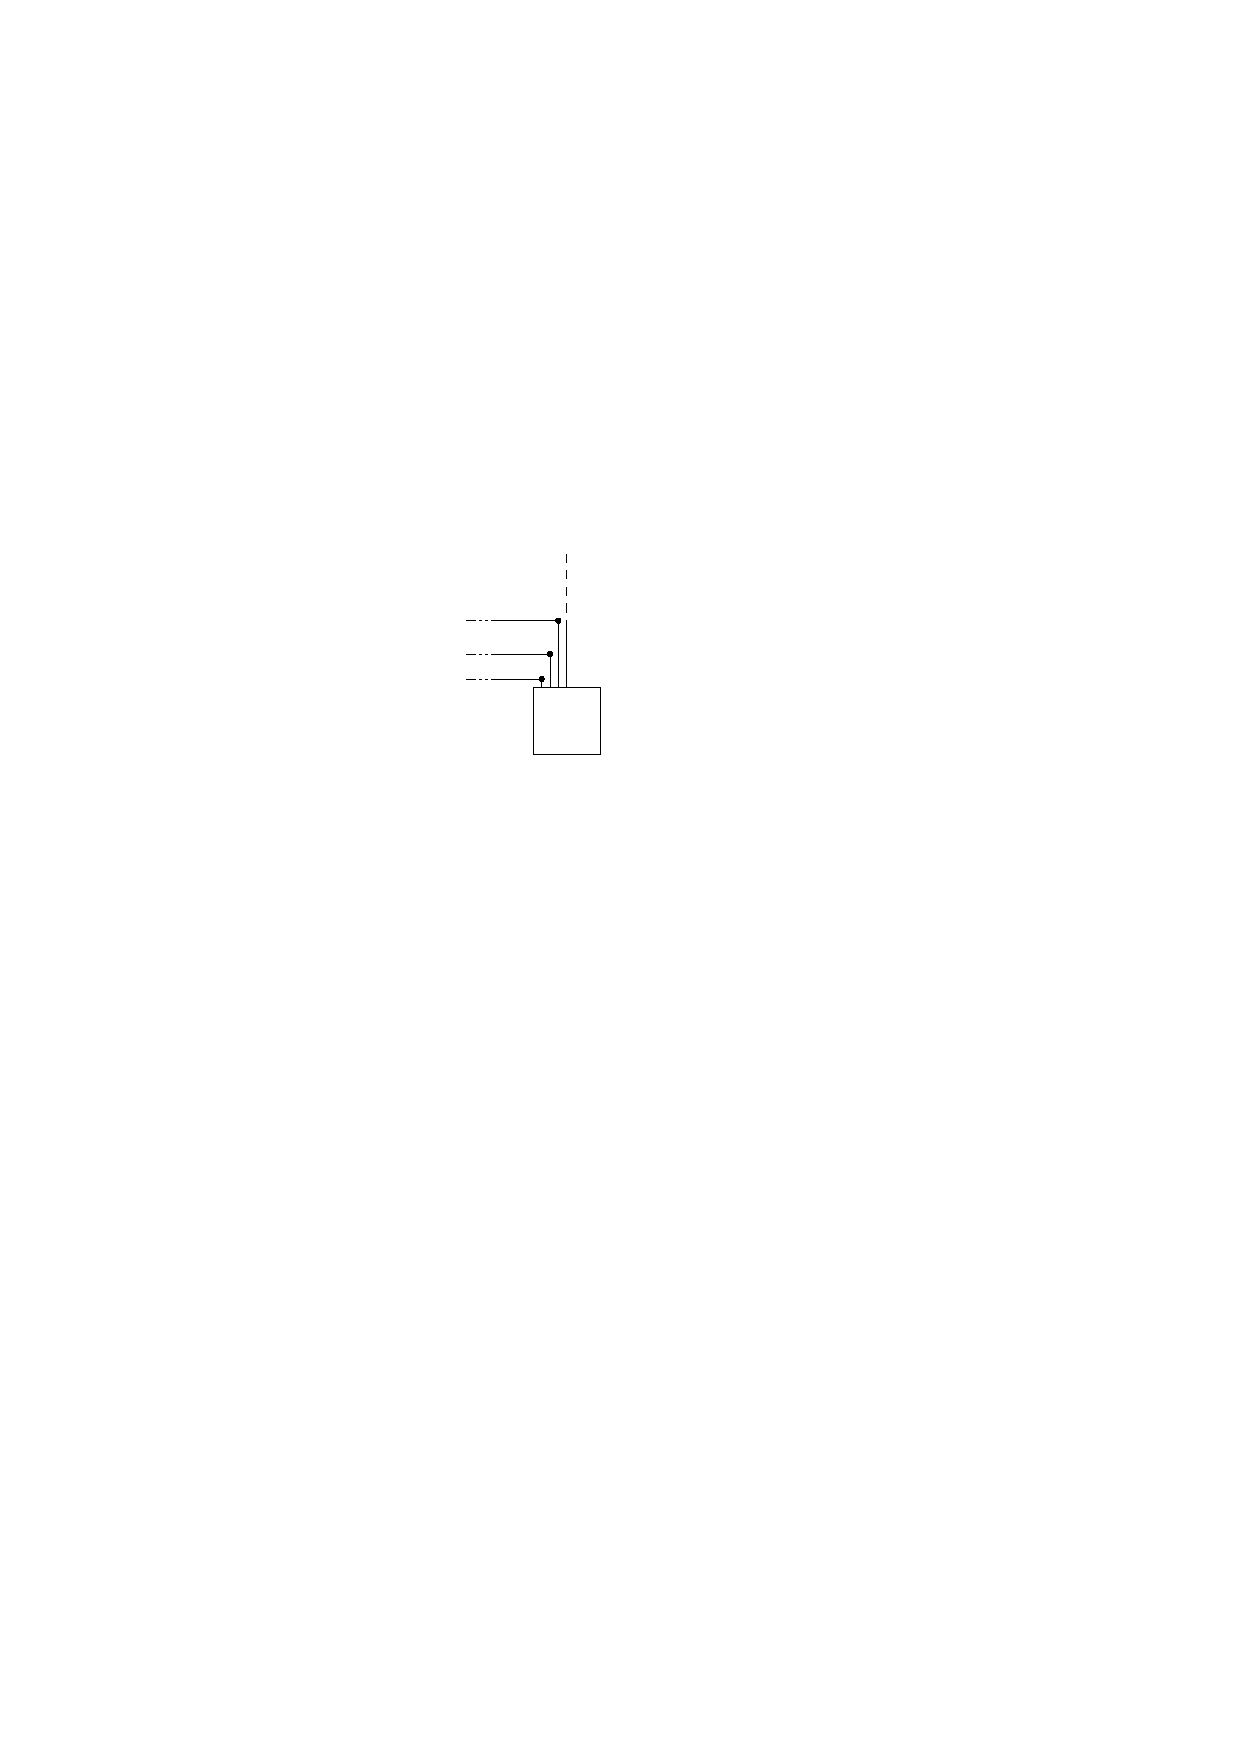
\includegraphics[width=0.55\linewidth,page=1]{includegraphics/1vertex-multEdges.pdf}
			\caption{Kandinsky situation}
		\end{subfigure}
	    \begin{subfigure}{0.3\textwidth}
		    \centering
		    \includegraphics[width=0.75\linewidth,page=2]{includegraphics/1vertex-multEdges.pdf}
		    \caption{}
	    \end{subfigure}
        \begin{subfigure}{0.3\textwidth}
	        \centering
	        \includegraphics[width=0.76\linewidth,page=3]{includegraphics/1vertex-multEdges.pdf}
	        \caption{SMOG representation}
        \end{subfigure}
        \caption{Smoothen multiple polyedges on the same port}
	\end{figure}
\\
The polyedges are connected equidistantly to a port. The increasing radii from outside-in and the original planarity in Kandinsky guarantee the planarity preservation of the resulting SMOG representation.	
\end{proof}
These results regarding graphs with arbitrary degree imply the functionality of the stretching technique even for the Kandinsky model. \cite[p. 582, Section 4.1]{SMOG}
\begin{corollary}
	Let $G$ be a graph with arbitrary degree and $\Gamma_G$ a planar orthogonal drawing in the Kandinsky model. Then, the stretching technique from \cite[p. 582, Section 4.1]{SMOG} is applicable guaranteeing the circular arc substitution. To be more precise, $\Gamma_G$ can be postprocessed to a SMOG representation, taking $\Rho(n^2) \times \Rho(n)$ area.
\end{corollary}
\begin{proof}
	The \textit{bend or end} property from Lemma \ref{lem:bend_or_end} and the Kandinsky bends in SMOG from Lemma \ref{lem:Kandinsky_bend} guarantee the preservation of the planarity and the necessary space for the circular arc substitution is given, as we can see in Lemma \ref{lem:space_stretch}. The worst case example drawing in the 4-planar situation regarding horizontal area bounds also takes effect in the $k$-planar situation.
	\begin{figure}[H]
		\centering
		\begin{subfigure}{0.4\textwidth}
			\centering
			\includegraphics[width=0.7\linewidth,page=3]{includegraphics/4-planar_worst_case.pdf}
			\caption{Original orthogonal graph}	
		\end{subfigure}
		\begin{subfigure}{0.6\textwidth}
			\centering
			\includegraphics[width=0.9\linewidth,page=4]{includegraphics/4-planar_worst_case.pdf}
			\caption{After applying the stretching technique}
		\end{subfigure}
		\caption*{Recall the worst case situation of Figure \ref{im:4-planar_worst_case}}
	\end{figure}
\end{proof}
\newpage
\subsection{Edge Complexity Investigation}
%The input will we a drawing of a graph in the Kandinsky Model, which means that there are only vertical and horizontal line segments, vertices illustrated in squares of a uniform size. Vertices lie on a course integer grid, while the line segment lie on a fine grid. The course grid is embedded in the fine grid.$$\text{Grid}_{\text{vertices}} \subset \text{Grid}_{\text{edges}}$$ A polyedge is an edge consisting of multiple line segments. The end of a line segment is either connected to another line segment or to a vertex. It is possible that multiple polyedges are connected to the same port of a vertex.\\
As we saw in the previous section, the possibility of a SMOG representation is given in the $k$-planar situation. All that remains is the examination regarding the number of bends of a polyedge. Previous results deliver an upper bound of the $4$-planar graphs by a cofactor of $\lceil\frac{3}{2}\rceil$ in the fixed shape model. We will see, that this upper bound still pertains.\\
Let $G$ be a planar graph with arbitrary degree, an orthogonal drawing $\Gamma_G$ is given and let $k$ describe the edge complexity of a polyedge of $\Gamma_G$. The main goal of this section is to examine lower and upper bounds for $k$ in SMOG.
%\begin{theorem}
%Let $\Gamma_G$ be an orthogonal drawing. Then: $$OC_{k+1} \hookrightarrow SC_{2k+1}$$ under the Fixed Layout Model.
%\end{theorem}
%\begin{proof}[Proof]
%Consider following graph:
%\begin{center}
%\texttt{TODO: Staircase graph}
%\end{center}
%As you can see, the upper bound is strict in this case due to the fix position of the vertices.
%\end{proof}
%\subsection{Fixed Shape Model}
%The only case where the new space is not guaranteed are vertical line segments ending in a vertex along with other vertical lines ending at the same port. We shall see that this will not be a problem regarding the edge complexity.\\
%In practice, the SMOG Model is derived from the Kandinsky Model using basically two plane sweeps: The first plane sweep stretches the Kandinsky drawing horizontally by the factor of the longest vertical line segment. The second plane sweep erases 90 degree bends by circular arc substitution, making the drawing \textit{smooth}. The resulting drawing is in $\Rho(n^2) \times \Rho(n)$ area due to the horizontal stretching.
\subsubsection{Examining \grqq good\grqq~and \grqq bad\grqq~parts of a polyline}
The general idea is to distinguish between two major cases: Line segments with alternating turns (staircase, zig-zags) and line segments with uniform turns (spirals, u-shapes). As we already saw, the SMOG representation of uniform turns does not increase the edge complexity. Therefore we examine polyedges regarding its properties of turns from one vertex to another. We will try to maximize the uniform part and simultaneously minimize the alternating part of a polyedge. We achieve this by so-called \textit{fragmentation} of a polyedge.
\begin{definition}
	An \textbf{edge fragment} is a non-empty sequence of line segments. A \textbf{fragmentation} of a polyedge is a sequence of fragments.
\end{definition}
The main advantage of the fragmentation is that every fragment can be seen as an independent polyedge.
The property of turns is crucial for the edge complexity thus the main criterion for the fragmentation.
\begin{definition}
	A fragment is pure in its turns; like in Definition \ref{def:uni_alt}, a fragment is uniform if and only if all turns share the same direction. A fragment is alternating if and only if the turns are all alternating.
\end{definition}
\begin{lemma} The fragmentation of a given polyedge $e$ is not unique.
\end{lemma}
\begin{proof}
	Consider the polyedge $(1,2)$ illustrated at Figure \ref{im:nonunique}. The algorithm \ref{algo:frag} takes the first three segments, considers its turn property and iterates along the polyedge. In the first picture, the segments starting from vertex 1 are obviously alternating, resulting in an uniform fragment consisting of only one segment. Similarily, starting at vertex 2, the first three fragments are uniform, the rest along to vertex 1 alternating. Both fragmentations are correct.
	\begin{figure}[H]
		\centering
		\begin{subfigure}{0.4\textwidth}
			\centering
			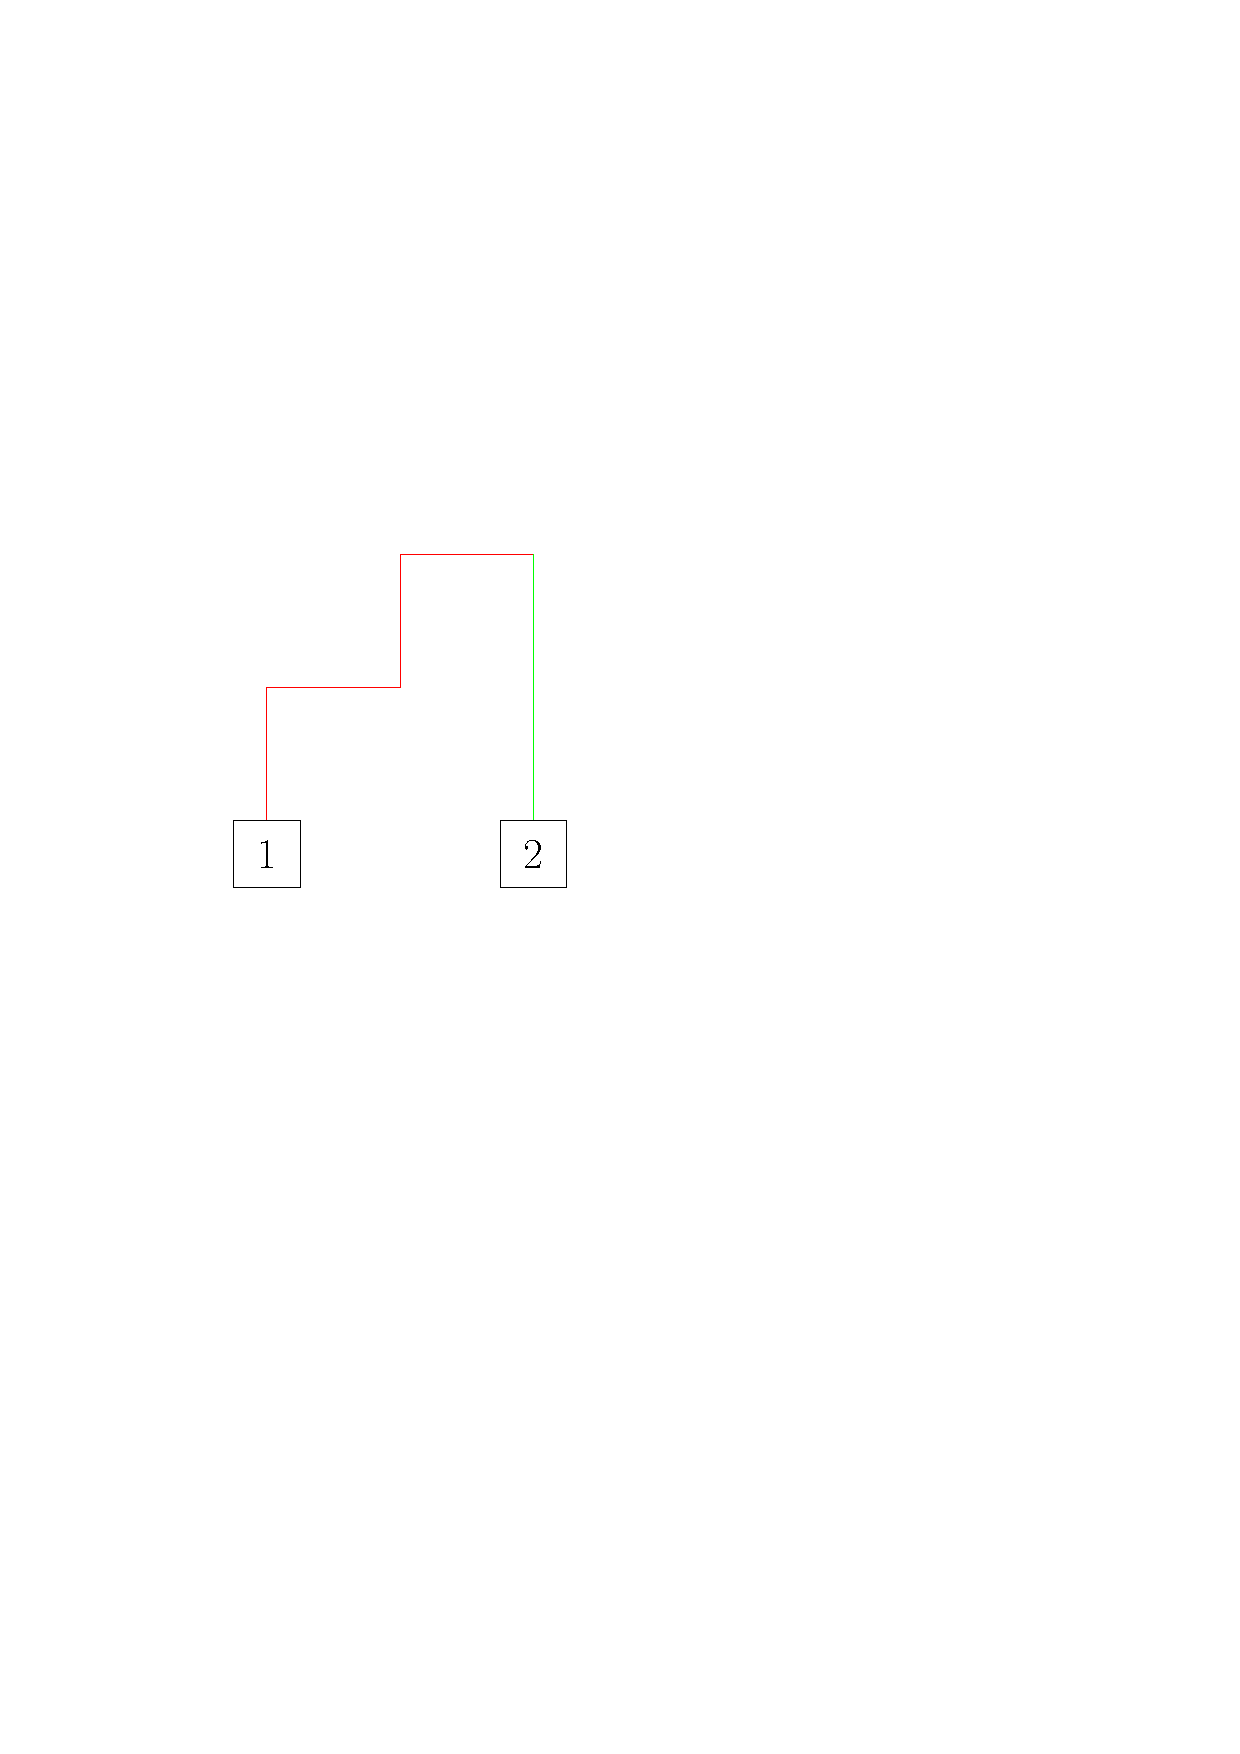
\includegraphics[width=0.6\linewidth,page=1]{includegraphics/non-unique-frag.pdf}
			\caption{Fragmented from $1$ to $2$}
		\end{subfigure}
		\begin{subfigure}{0.4\textwidth}
			\centering
			\includegraphics[width=0.6\linewidth,page=2]{includegraphics/non-unique-frag.pdf}
			\caption{Fragmented from $2$ to $1$}
		\end{subfigure}
		\caption{Non-unique fragmentation}\label{im:nonunique}
	\end{figure}
\end{proof}
\begin{definition}
	Let $e'$ and $f'$ be two fragmentations. Then 
	\begin{align*}e' \thicksim_R f' \Leftrightarrow \Gamma_{e'} = \Gamma_{f'}
	\end{align*}\label{def:frag_relation}
\end{definition}
This means that two fragmentations are relative if and only if they describe the same polyedge in a given drawing.
\begin{lemma}
	The relation from Definition \ref{def:frag_relation} is an equivalence relation.
\end{lemma}
\begin{proof}
	Describing the same image is trivially reflexive, symmetical and transitive.
\end{proof}
\begin{definition}
	Two fragments $f$ and $g$ are called incompatible if any segment transfer between $f$ and $g$ result in a turn property collision.
\end{definition}
\begin{figure}[h]
	\centering
	\begin{subfigure}{0.4\textwidth}
		\centering
		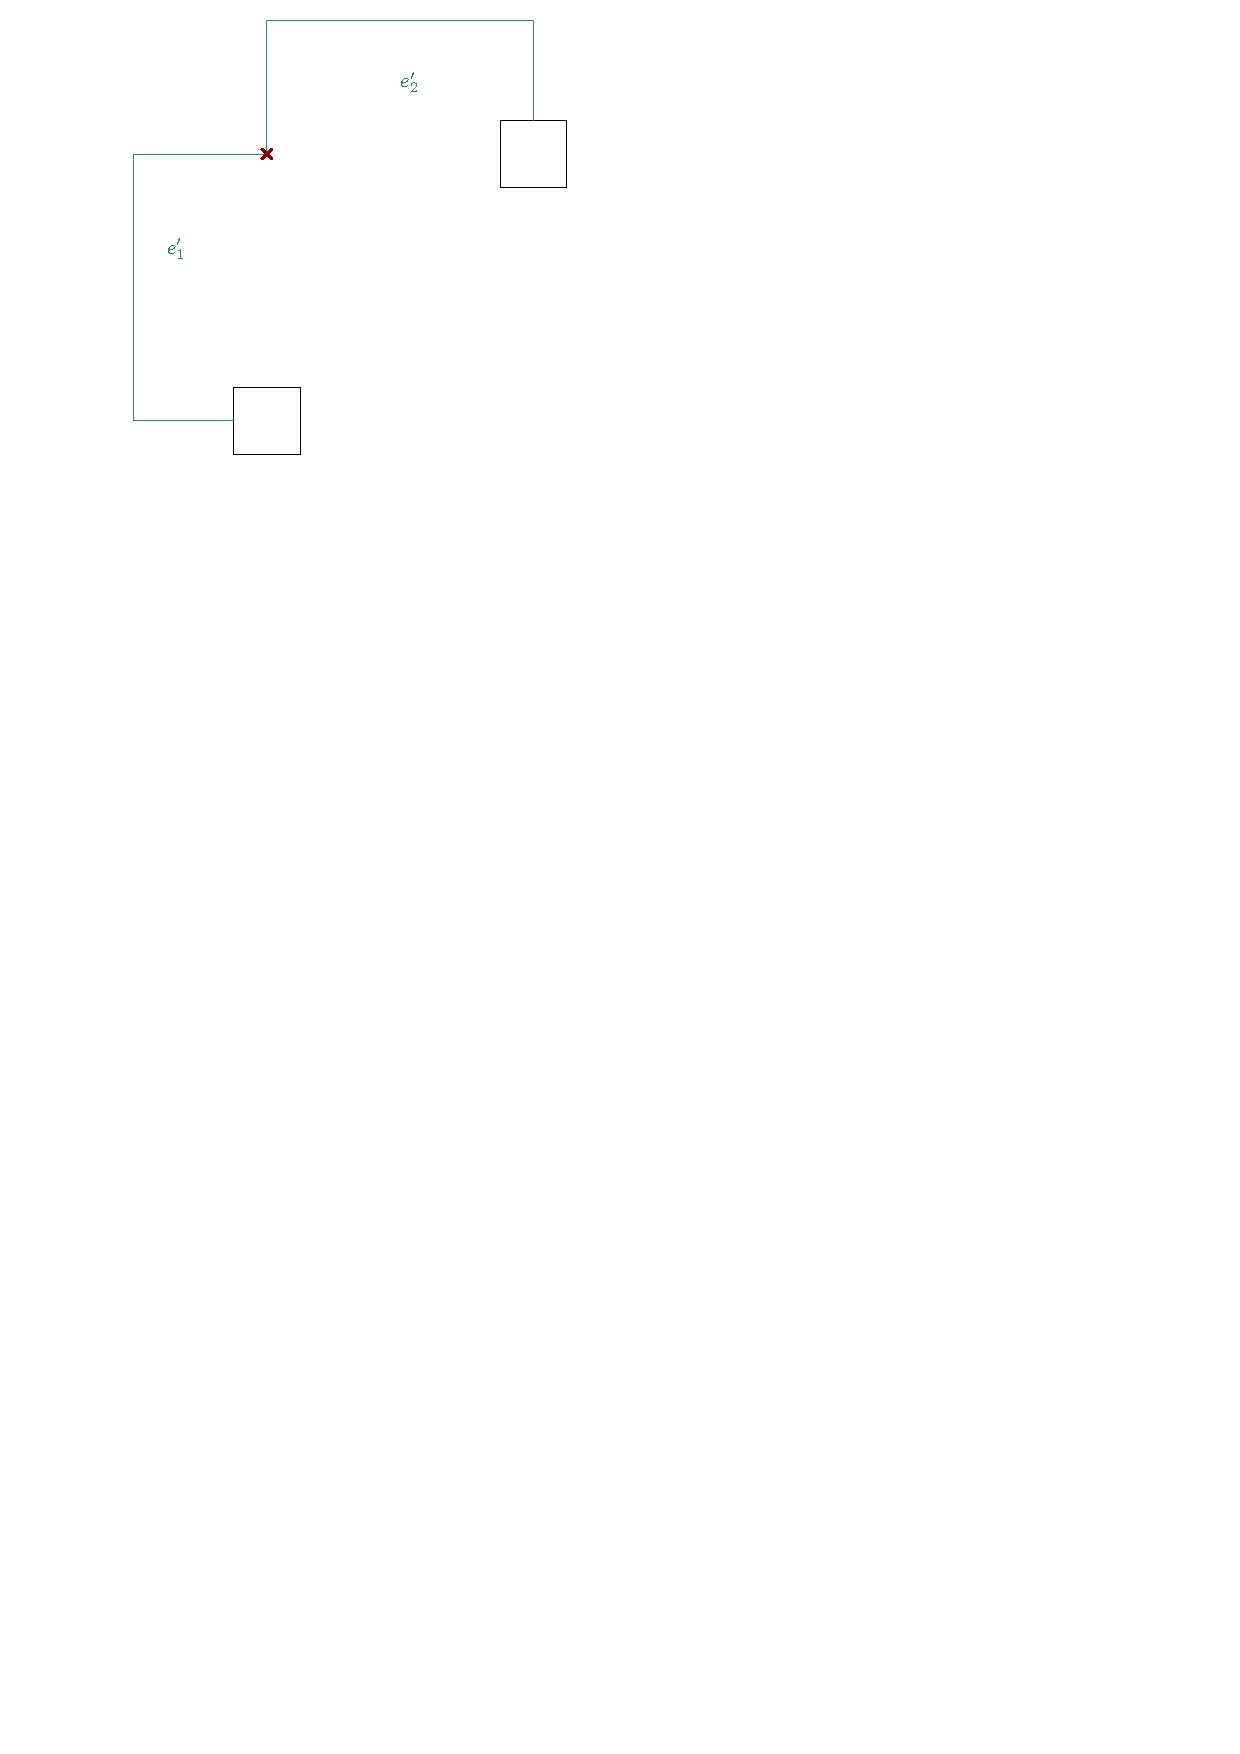
\includegraphics[width=0.7\linewidth,page=1]{includegraphics/unmergable_frags.pdf}
	\end{subfigure}
	\caption{Incompatible uniform fragments $e'_1,e'_2$}\label{im:incompatible}
\end{figure}
What if the polyedge we want to fragment inherits an edge complexity of at most 2? Fragmentation is meant to partition large polyedges but the small case still has to be considered. 
\begin{lemma}
	Fragments of length up to two are simultaneously uniform and alternating. For a definite statement, those fragments lack in the third segment.\label{lem:2-frag}
\end{lemma}
When we encounter a fragment of length two, we will interpret it as a uniform fragment first since uniformity does not necessarily increase the complexity. So now we are able to create a first - rather naive - algorithm in order to find a valid fragmentation.\newpage
\begin{algorithm}[H]
	\KwIn{Polyedge $e$ with edge complexity $k,k\geq 2$}
	\KwResult{$e'$, a first fragmentation of $e$}
	\If{$k = 2$}{
		$e'_1\gets (e_1,e_2)$\\
		$e'_1.\texttt{uniform = true}$\\
		$e' \gets (e'_1)$
	}
	\Else{
		$e'_1 \gets (e_1,e_2,e_3)$\\
		$e' \gets \emptyset$\\
		$i \gets 1$\\
		\If{$e'_1$ uniform}{$e'_1.\texttt{uniform} = \texttt{True}$}
		\Else{$e'_1.\texttt{uniform} = \texttt{False}$}
		\For{$j = 4$ to $k$}{
			\If{$e_j$ fits into the turn property of $e'_i$}{
				$e'_i.\texttt{append}$($e_j$)
			}
			\Else{
				%create a new fragment with $e'_m.\texttt{uniform} \gets \neg e'_{m-1}.\texttt{uniform}$ and continue
				$e'.\texttt{append}(e'_i)$\\
				$i \gets i + 1$\\
				$e_i.\texttt{uniform} = \neg e_{i-1}.\texttt{uniform}$\\
				$e_i \gets (e_j)$
			}
		}
	}
	$e'.\texttt{append}(e'_i)$\\
	\Return $e'$
	\caption{\texttt{fragment\_naively}$(e) \in \Rho(k)$}\label{algo:frag}
\end{algorithm}
\subsubsection{Correctness of algorithm \ref{algo:frag}}
This algorithm works for polyedges of length at least two. If the length is two, then the fragmentation will be unique since a fragment of length two is both uniform and alternating due to Lemma \ref{lem:2-frag}. If the complexity of the polyedge is greater than two, then lines 6 to 12 initialize the first fragment of length three and determines its turn property. For the remaining segments, this algorithm tests whether the next segment fits into the current fragment and appends it, if that is the case. If not, then the current fragment is appended to the returning fragmentation and a new fragment is created with the opposite turn property. By testing for every segment if it fits into the current fragment, this algorithm returns a valid fragmentation and runs in $\Rho(k)$.\\
\\We will see in the following lemma, that this algorithm should be improved.
\begin{lemma}
	Algorithm \ref{algo:frag} is not sufficient to determine a satisfying fragmentation.
\end{lemma}
\begin{proof}
	Consider following polyedge given in \ref{im:bad_frag}. By applying algorithm \ref{algo:frag}, we achieve the following fragmentation. Green fragments illustrate uniform ones, red ones illustrate alternating ones. Red dots illustrate the breaking point in the fragment creation.
	\\
	\begin{figure}[h]
		\centering
		\begin{subfigure}{0.3\textwidth}
			\centering
			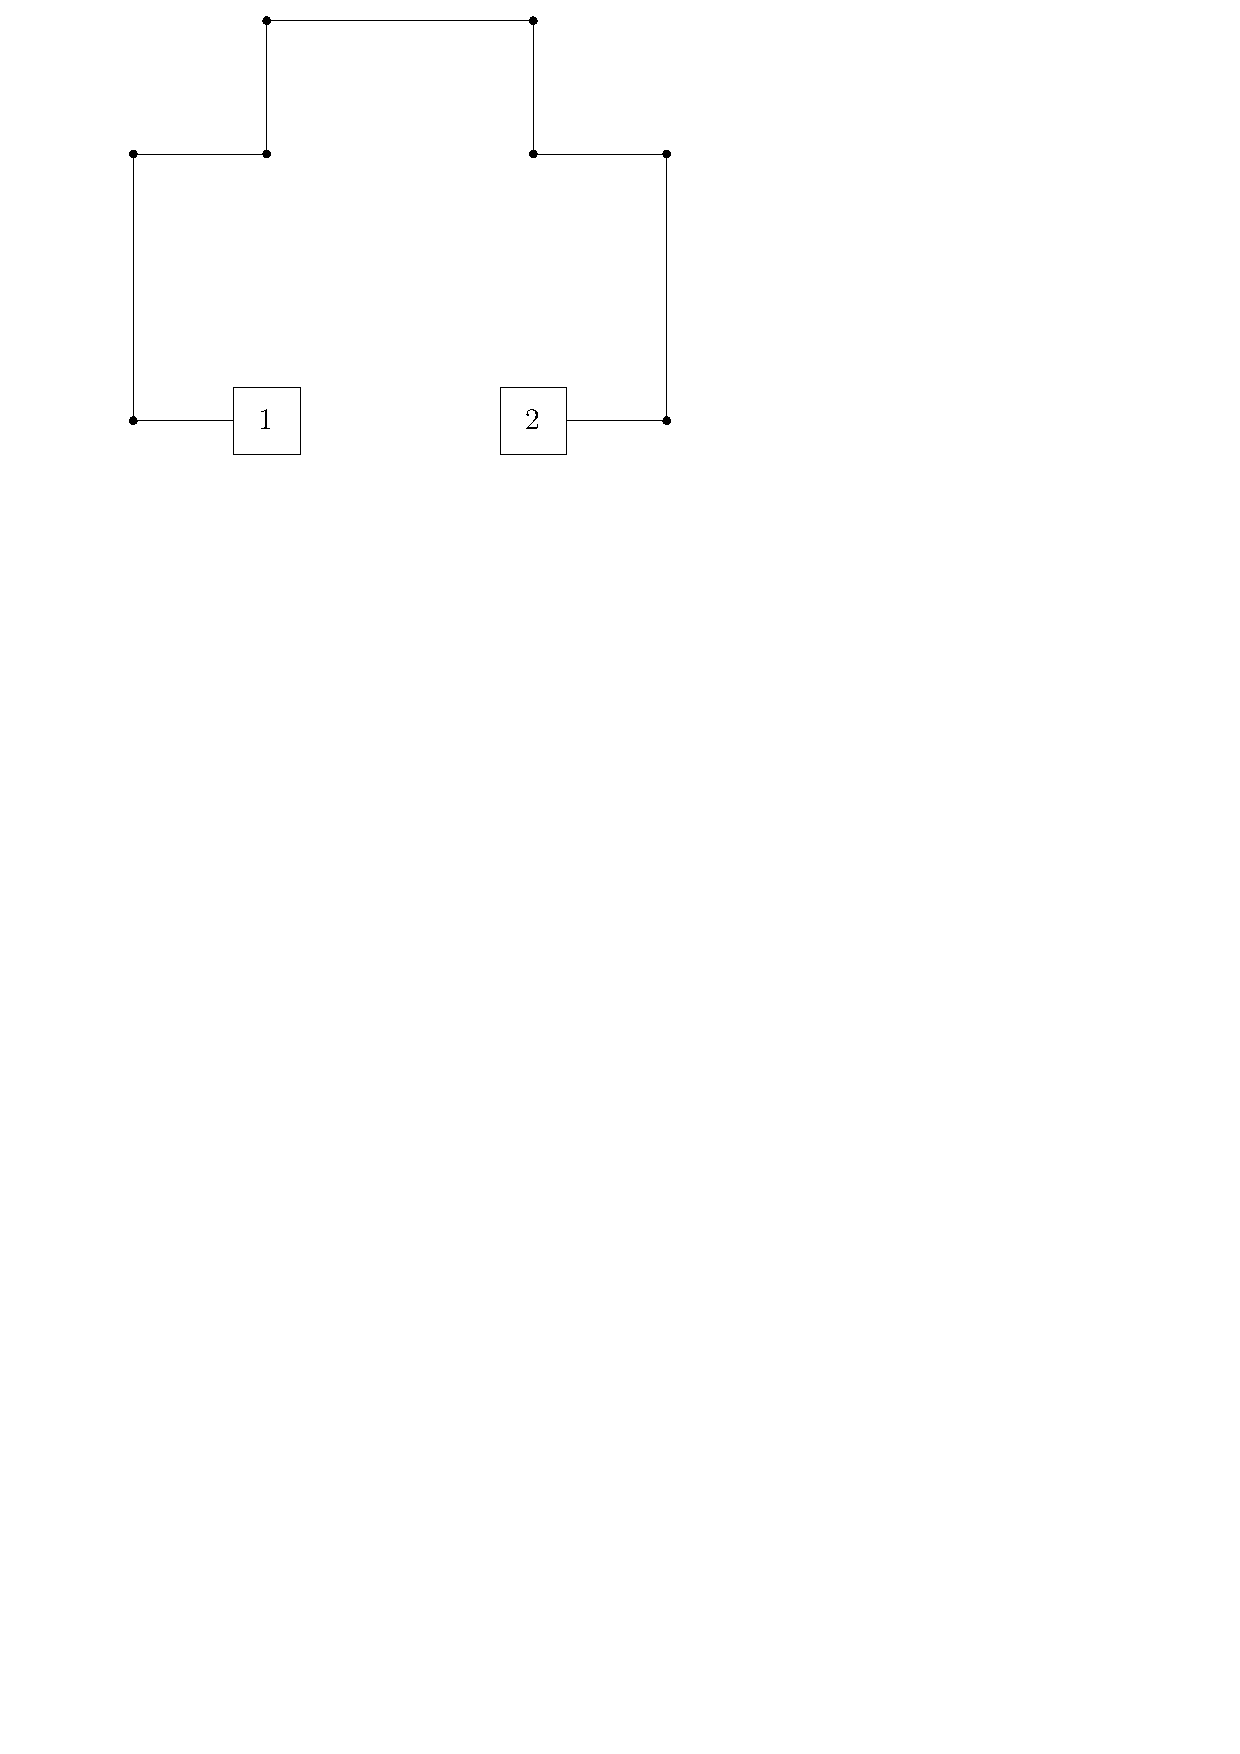
\includegraphics[width=0.7\linewidth,page=1]{includegraphics/bad_fragmentation.pdf}
			\caption{original input polyedge}\label{im:bad_frag1}
		\end{subfigure}
		\begin{subfigure}{0.3\textwidth}
			\centering
			\includegraphics[width=0.7\linewidth,page=2]{includegraphics/bad_fragmentation.pdf}
			
			\caption{Result of algorithm \ref{algo:frag}}\label{im:bad_frag2}
		\end{subfigure}
		\begin{subfigure}{0.3\textwidth}
			\centering
			\includegraphics[width=0.7\linewidth,page=3]{includegraphics/bad_fragmentation.pdf}
			
			\caption{more appreciating result}\label{im:bad_frag3}
		\end{subfigure}
		\caption{Bad example of a polyedge for the first approach}
		\label{im:bad_frag}
	\end{figure}
	\\
	As we can see in \ref{im:bad_frag2}, algorithm \ref{algo:frag} delivers a fragmentation which consists of multiple fragments of length two. That is because algorithm \ref{algo:frag} forces two consecutive fragments to differ in their turn property. As we know from Lemma \ref{lem:2-frag}, fragments of length two are not that conclusive in this case. The result given in \ref{im:bad_frag3} consists of longer fragments and seems to be somehow more precise regarding the polyedge. The big difference lies in the abortion of the change constraint regarding consecutive fragments.
\end{proof}
How do we find the best way to describe a polyedge as a fragmentation? One way to approach it is to minimize the total number of fragments and the number of alternating fragments. This leads to the following ordering relation:
\begin{lemma}
	The amount of all possible fragmentations of a polyedge $e$ is finite. To be more precise: $$|[e]_{\thicksim_R}| < 2^{k^2}$$
\end{lemma}
\begin{proof}
	Given a polyedge $e$, the amount of possible fragments $s$ is computed:
	\begin{align*}
	s &\leq \sum_{i=1}^k \frac{k}{i} \cdot i = k^2
	\end{align*}
	$i$ illustrates the length of the fragments starting from $1$ to $k$. Consider $e$ partitioned into $\frac{k}{i}$ fragments, then there are $\leq i$ ways to start the fragmentation. The offset lies in $[0,i-1]$. The cardinality of the power set containing all possible fragments values $2^{k^2}$.
\end{proof}
As we already saw, there are multiple ways to describe a polyedge regarding a fragmentation. The next step is to determine, which fragmentation suits the best. Given a mathematical backbone to a given polyedge $e$, we want to describe the \grqq best way\grqq~to determine the number of bends in SMOG. So we will pick the \grqq best\grqq~fragmentation, which will be minimal in its number of alternating fragments and minimal in its total number of fragments.
\begin{definition}\label{def:ord_rel}
	Let $e',f'$ be two fragmentations of the same polyedge $e$ ($e' \thicksim_R f'$). Then we define a relation:
	\begin{align*}
	e' \leq f' \Leftrightarrow \left(\#_{\text{altFrag}}(e') \leq \#_{\text{altFrag}}(f')\right) \wedge \left(\#_{\text{totalFrag}}(e') \leq \#_{\text{totalFrag}}(f')\right)
	\end{align*}
\end{definition}
\begin{lemma}
	The relation from Defintion \ref{def:ord_rel} is sufficient to determine a minimum of $[e]_{\thicksim_R}$. 
\end{lemma}
\begin{proof}
	Obviously, the relation $\leq$ is reflexiv and transitive. Therefore, this relation is a preorder and we are able to determine a minimum of $[e]_{\thicksim_R}$ because in a finite set there is a minimum regarding a preorder.
\end{proof}
Comparing all possible fragmentations for the minimum will result in an exponential runtime. In order to fix this problem, we will take a slightly different approach - we will further get rid of alternating fragments by creating uniform-only fragments. This will result in longer fragmentations at first but we will see that it will be acceptable due to a new interpretation of this fragmentation.\\
Using Lemma \ref{lem:2-frag}, we will be able to substitute alternating fragments as a sequence of uniform fragments.
\begin{lemma}
	A fragment $f$ of length $k'$ is alternating if and only if its purely uniform fragmentation $f'$ of size $\left\lceil\frac{k'}{2}\right\rceil$ inherits uniform incompatible fragments of length 2 and $f \thicksim_R f'$ regarding definition \ref{def:ord_rel}. This enables us to distinguish uniform fragments from alternating ones in the output of algorithm \ref{algo:2ndfrag}.\label{lem:alt_2uni}
\end{lemma}
\begin{proof}
	If a fragment $f$ of length $k'$ is alternating, then every bend differs in its direction regarding the previous one. A fragment of length 2 inherits one bend. In an alternating fragment, the next one will cause a turn property collision, resulting in a new fragment. Again, fragments of lengths up to 2 are uniform by definition. Similarily, consider a sequence of fragments of length 2. If there were an optimization possible, then the sequence would not be completely incompatible as stated. This implies the staircase situation.
\end{proof}
We are willing to lengthen the fragmentation by coincidentally describing more precisely. This leads to a modification of algorithm \ref{algo:frag}.\\
\begin{algorithm}[H]
	\KwIn{Polyedge $e$ with edge complexity $k$,$k\geq 2$}
	\KwOut{Almost optimal fragmentation of $e$}
	$e'_1 \gets (e_1,e_2)$\\
	$f \gets \emptyset$\\
	$i \gets 1$\\
	\For{$j = 3$ to $k$}{
		\If{$e'_i.\texttt{append}(e_j)$ is uniform}{
			$e'_i.\texttt{append}(e_j)$
		}
		\Else{
			$f.\texttt{append}(e'_i)$\\
			$i \gets i+1$\\
			$e'_i\gets (e_j)$
		}
		
	}
	$f.append(e'_i)$\\
	\texttt{Recheck}$(f)$\label{algo:2ndfrag_recheck}\\
	\Return $f$
	\caption{\texttt{fragment\_uniform-only}$(e)$ $\in \Rho(k)$}\label{algo:2ndfrag}
\end{algorithm}
\subsubsection{Correctness of algorithm \ref{algo:2ndfrag}}
This algorithm is pretty similar to algorithm \ref{algo:frag} with the big difference, that every fragment is now uniform. Initializing $f$ as a list of fragments, this algorithm appends the current fragment if the next segment collides with its turn property. Unless there is only one segment left in the end, every fragment consists of at least two segments. On the other side, there are optimal fragmentations which inherit a fragment of length one. Consider algorithm \ref{algo:2ndfrag} without line \ref{algo:2ndfrag_recheck}.
\begin{figure}[H]
	\centering
	\begin{subfigure}{0.3\textwidth}
		\centering
		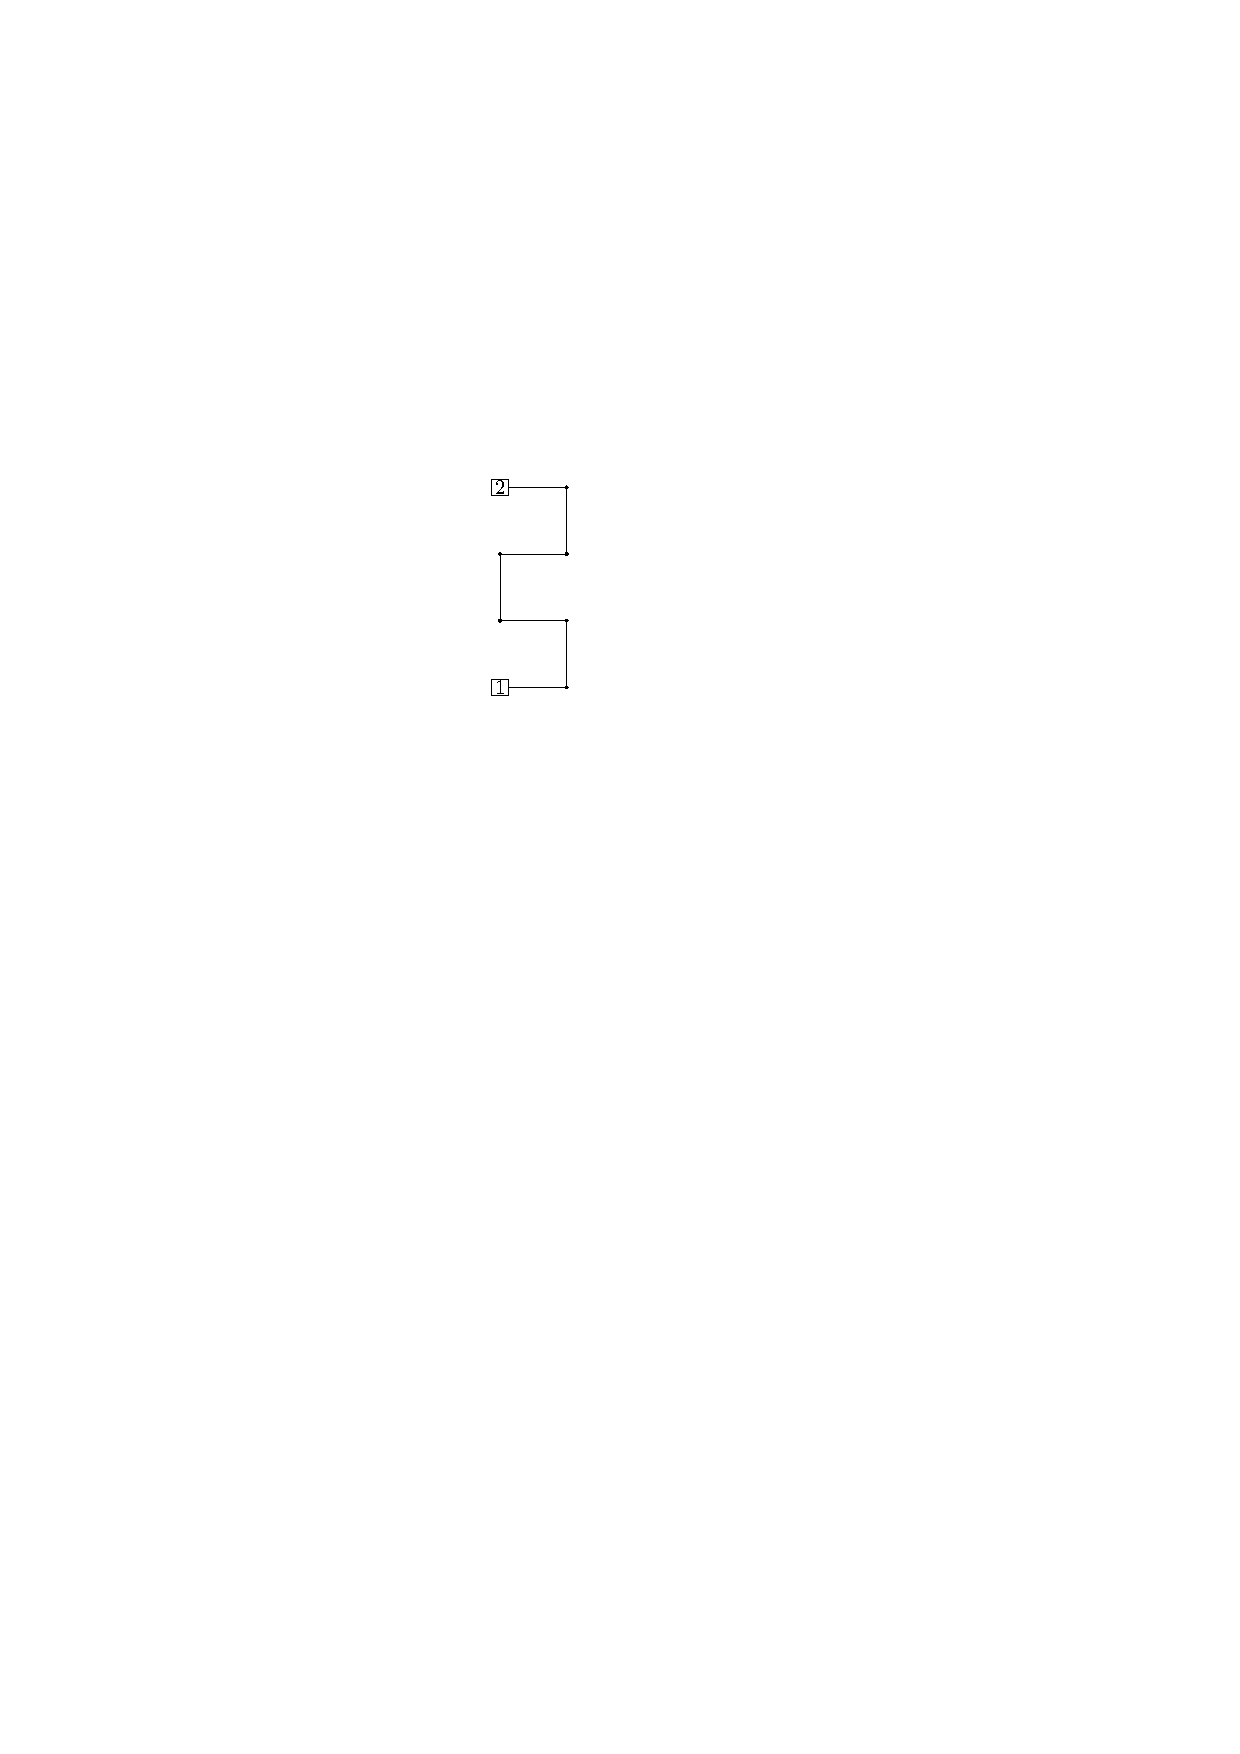
\includegraphics[width=0.4\linewidth,page=1]{includegraphics/bad_2ndfrag.pdf}
		\caption{original input polyedge}\label{im:bad_2ndfrag1}
	\end{subfigure}
	\begin{subfigure}{0.3\textwidth}
		\centering
		\includegraphics[width=0.4\linewidth,page=2]{includegraphics/bad_2ndfrag.pdf}
		
		\caption{Result of algorithm \ref{algo:2ndfrag}}\label{im:bad_2ndfrag2}
	\end{subfigure}
	\begin{subfigure}{0.3\textwidth}
		\centering
		\includegraphics[width=0.4\linewidth,page=3]{includegraphics/bad_2ndfrag.pdf}
		\caption{more appreciating result}\label{im:bad_2ndfrag3}
	\end{subfigure}
	\caption{Bad example of a polyedge for the second uniform-only approach (red highlights the problematic fragment)}
	\label{im:bad_2ndfrag}
\end{figure}
In figure \ref{im:bad_2ndfrag} the output of algorithm \ref{algo:2ndfrag} returns uniform-only fragments. The colour highlighting is used this time to illustrate the problem description. In Figure \ref{im:bad_2ndfrag2}, we see that the length of the fragments equals $(3,2,2)$, whereas in Figure \ref{im:bad_2ndfrag3} the individual length is $(3,1,3)$. We are still almost there, although there are situations, where the \grqq bad\grqq~part of a fragmentation is of length one. Still, algorithm \ref{algo:2ndfrag} functions the way we want to. We only have to \textit{recheck} the fragmentation (Line \ref{algo:2ndfrag_recheck} in algorithm \ref{algo:2ndfrag}), whether a fragment of length two can be further minimized by merging the last segment with the next fragment.\\
\begin{algorithm}[H]
	\KwIn{A fragmentation $f$}
	\KwOut{A fragmentation $f$ rechecked}
	\caption{\texttt{recheck}$(f) \in \Rho(k)$\label{algo:recheck}}
	\For{$i = 1$ to $f$\texttt{.length}$-1$}{
		\If{$f_i$.\texttt{length} $= 2$}{
			$v \gets$ first segment of $f_i$\\
			$u \gets$ second segment of $f_i$\\
			\If{$(u)\texttt{.append}(f_{i+1})$\texttt{.uniform} = \texttt{true}}{
				$f_i \gets (v)$\\
				$f_{i+1} \gets (u).\texttt{append}(f_{i+1})$
			}
		}			
	}
	\Return $f$
\end{algorithm}
Obviously, this algorithms runtime is linear to the edge complexity of the input orthogonal polyedge.
\begin{theorem}
	Algorithm \ref{algo:2ndfrag} is sufficient to determine the edge complexity of any polyedge in the smooth orthogonal drawing. Furthermore, the resulting fragmentation can be used to describe a polyedge adequately.
	\label{th:2ndfrag}
\end{theorem}
\begin{proof}
	We already know that uniform fragments do not increase in their complexity and the transition between two incompatible fragments increases the complexity by 1. This leads to a new computation regarding the edge complexity of any polyedge in the smoothened drawing:
	\begin{align}
	ec(f) = \sum_{i = 1}^{f.\texttt{length}} ec(e'_i) + \underbrace{(f.\texttt{length} - 1)}_{\text{fragment transitions}}\label{eq:2ndfrag}
	\end{align}
	The information of alternating fragments does not get lost. By substituting consecutive fragments of up to length two with one big alternating fragment, we are able to describe the behaviour of the polyedge adequately.
\end{proof}
Now we want to establish an algorithm which modifies the fragmentation resulted from algorithm \ref{algo:2ndfrag} to describe the minimum.\\
\begin{algorithm}[H]
	\KwIn{Fragmentation $f$ computed by algorithm \ref{algo:2ndfrag} and \ref{algo:recheck}}
	\KwOut{Minimal fragmentation $e_{\min}$ regarding the relation {\ref{def:ord_rel}}}
	\caption{Min computing of all the fragmentations regarding relation {\ref{def:ord_rel}} \label{al:min_computing}}
	
	$e_{\min} \gets \emptyset$\\
	$f_{\text{alt}} \gets \emptyset$\\
	$f_{\text{alt}}\texttt{.uniform} = \texttt{false}$\\
	\For{$i = 1$ to $f\texttt{.length}$}{
		\If{$f_i\texttt{.length} \geq 3$}{
			\If{$f_\text{alt} \neq \emptyset$}{
				$e_{\min}\texttt{.append}(f_\text{alt})$\\
				$f_\text{alt} \gets \emptyset$
			}
			$f_i\texttt{.uniform} = \texttt{true}$\\
			$e_{\min}\texttt{.append}(f_i)$		
		}
		\Else{
			$f_\text{alt}\texttt{.append}(f_i)$
		}
	}
	\If{$f_\text{alt} \neq \emptyset$}{
		$e_{\min}\texttt{.append}(f_\text{alt})$\\
		$f_\text{alt} \gets \emptyset$
	}
	\Return $e_{\min}$
\end{algorithm}
\subsubsection{Correctness of algorithm \ref{al:min_computing}}
This algorithm gets the uniform-only fragmentation from algorithm \ref{algo:2ndfrag} as input and determines whether a fragment is of length greater than two. If so, then this fragment is purely uniform and can be considered that way. However, if a fragment is of length one or two, these segments did not fit in any other uniform fragment due to collision reasons. They can be considered as alternating. By using Lemma \ref{lem:alt_2uni}, we know that consecutive fragments of length at most two are analogous to an alternating fragment. This algorithm merges those consecutive segments initialized in line 2-3 and appends them, if a consecutive fragment is of length at least three or there are no further fragments left at the end of the \texttt{for} loop. The longest possible fragmentation given by algorithm \ref{algo:2ndfrag} is of length $\left\lceil\frac{k}{2}\right\rceil$, where $k$ is the complexity of the original orthogonal polyedge and therefore this algorithm also terminates in $\Rho(k)$ runtime.
\begin{theorem}
	The fragmentation resulting from algorithm \ref{algo:2ndfrag} and \ref{al:min_computing} describes a minimal fragmentation regarding the relation \ref{def:ord_rel}.\label{th:frag_min}
\end{theorem}
\begin{proof}[Proof by contradiction]
	Let $e_{\min}$ be the result of algorithms \ref{algo:2ndfrag} and \ref{al:min_computing} and $f_{\min}$ be the another valid fragmentation regarding the relation \ref{def:ord_rel}. Assume that $f_{\min} < e_{\min}$. This would mean that the number of total fragments in $f_{min}$ would be less and the number of alternating fragments are at most the same. This would mean there would be a fragment which can be split into the at most two consecutive fragments. Since algorithm \ref{algo:2ndfrag} merges uniform ones as long as possible and algorithm \ref{al:min_computing} merges alternating ones as long as possible, there is no possibility that this fragment could not have been saved beforehand. The same argument values for the case that $f_{\min}$ would have less alternating fragments. So $f_{\min} \nless e_{\min}$.
\end{proof}
The only thing left to consider is the uniqueness of the computed minimum. We will see that the fragmentations can differ if we change the direction of fragmentation.
\begin{lemma}
	Let $e = (1,2)$ be a polyedge. Then, the optimal fragmentation started at vertex 1 may differ from the fragmentation started at vertex 2.
\end{lemma}
\begin{proof}
	Consider the following example.
	\begin{figure}[H]
		\centering
		\begin{subfigure}{0.3\textwidth}
			\centering
			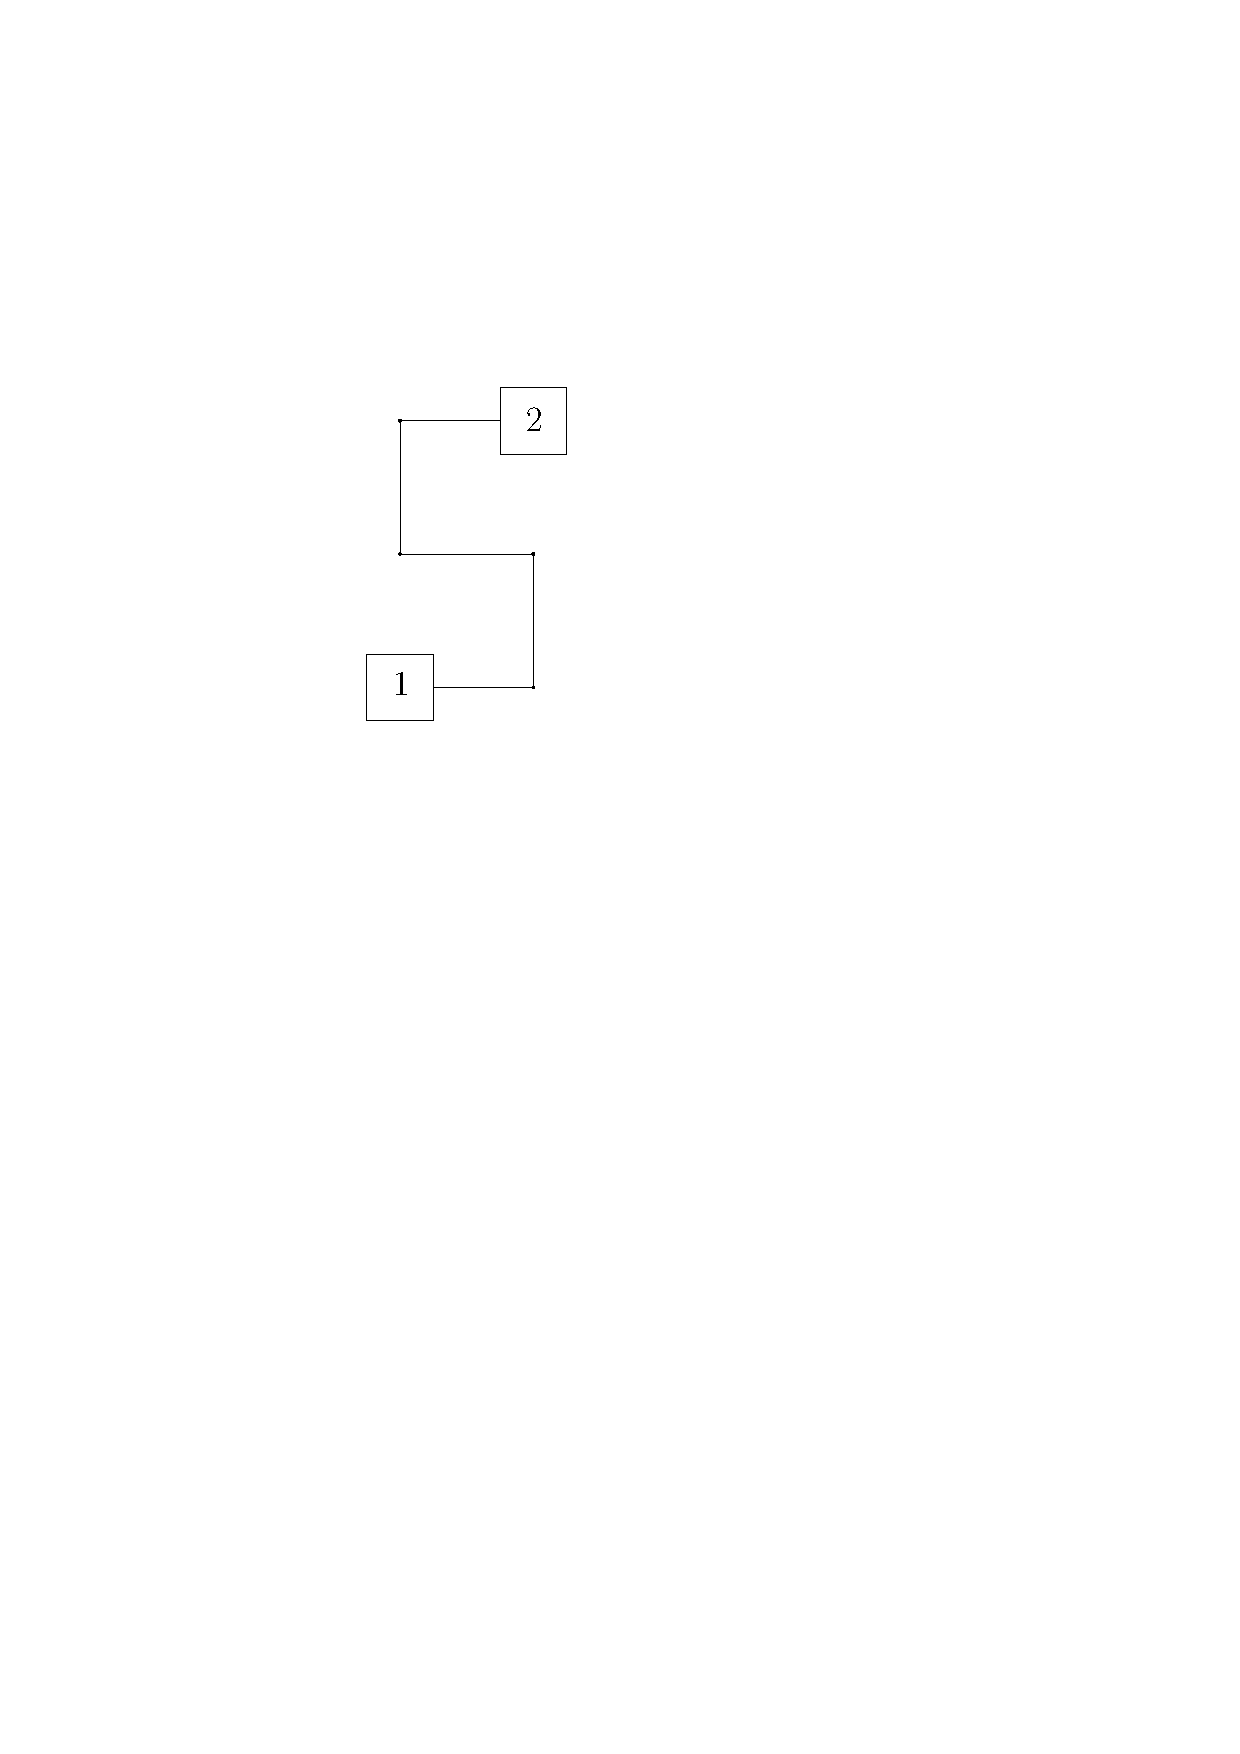
\includegraphics[width=0.4\linewidth,page=1]{includegraphics/non-unique-min.pdf}
			\caption{Input polyedge $(1,2)$}
		\end{subfigure}
		\begin{subfigure}{0.3\textwidth}
			\centering
			\includegraphics[width=0.4\linewidth,page=2]{includegraphics/non-unique-min.pdf}
			\caption{Fragmented from 1 to 2}
		\end{subfigure}
		\begin{subfigure}{0.3\textwidth}
			\centering
			\includegraphics[width=0.4\linewidth,page=3]{includegraphics/non-unique-min.pdf}
			\caption{Fragmented from 2 to 1}
		\end{subfigure}
	\caption{Non-unique optimal fragmentation regarding direction}\label{im:non-unique-min}
	\end{figure}
The fragmentation from 1 to 2 starts with an uniform fragment of length three, which is not contained in the fragmentation the other way around.
\end{proof}
We see, that the fragmentation is still pretty similar. The next lemma holds the uniqueness of the minimal fragmentation in sense of direction and that the choice of direction does not matter for the validity.
\begin{lemma}
	The fragmentation resulting from algorithm \ref{algo:2ndfrag} and \ref{al:min_computing} is the unique minimum with respect to the direction of the fragmentation. The two minima regarding both fragmentation directions share the same property regarding the number of (alternating) fragments.
\end{lemma}
\begin{proof}
	Consider two fragmentations $f_1$ and $f_2$ regarding the same polyedge $e$, both computed reciprocally with algorithm \ref{algo:2ndfrag} and \ref{al:min_computing}. Then, theorem \ref{th:frag_min} holds and the number of alternating fragments and the total number of fragments are of the same size. However, as we saw in figure \ref{im:non-unique-min}, the fragmentation itself can differ. 
\end{proof}
Now we achieved the best mathematical description of a polyedge in form of a fragmentation. This goes along pretty well with the already achieved results. The results of purely uniform or purely alternating polyedges also apply for purely uniform or purely alternating fragments because every fragment can be considered as a seperate polyedge simulated with dummy vertices. We will see that a fragment with edge complexity $k'$ can be transferred to a SMOG fragment with edge complexity $\leq \lfloor\frac{3}{2}k'\rfloor$. In fact, we will also see that every fragmentation with complexity $k'$ will result in a SMOG polyedge with complexity $\leq \lfloor\frac{3}{2}k'\rfloor$.
\subsection{Results}
In order to talk about the edge complexity of SMOGs drawings with arbitrary degree we have to consider the number of bends of the polyedges in SMOG. In this section we will look at the possible length of fragmentations, the merge of two fragmentations resulting in one extra bend and will summarize the results.
%\begin{lemma}
%Let $e$ be a polyedge and $e'$ its best fragmentation regarding the number of alternating fragments and total fragments. To be more precise: $e' = \min_{\leq}[e]_{\thicksim_R}$. If the polyedge $e$ does not have a minimal number of bends, $e'$ contains more than one fragment.
%\end{lemma}
\begin{lemma}
	Let $e$ be a polyedge with edge complexity $k$. Then the range of fragmentation lengths is bounded by $\left\lceil\frac{k}{2}\right\rceil$. To be more precise: $$ |e'| \in \left\{1,..., \left\lceil\frac{k}{2}\right\rceil\right\}~~~\forall e'\in [e]_{\thicksim_R} $$
\end{lemma}
\begin{proof}
	If a polyedge with complexity $k$ is purely alternating, then algorithm \ref{algo:frag} will return a valid fragmentation consisting of a single alternating fragment whereas algorithm \ref{algo:2ndfrag} will return a valid fragmentation of $\left\lceil\frac{k}{2}\right\rceil$ fragments. It is possible, that this last fragment is of length one.% or uniform, the minimum fragmentation length of 1 is trivial. Consider the algorithm \ref{algo:frag} given to find a worst case fragmentation. The idea is to create a new fragmentation whenever possible. The first fragment will be of length 3 (initialization of the algorithm), deciding the turn property. The next fragment will get the opposite turn property but will only inherit two segments since the third one will cause a new fragment. The algorithm terminates with either a 2-tuple fragment or a 1-tuple fragment to append. Therefore, there will be at most $\left\lceil\frac{k}{2}\right\rceil$ fragments.
	
	%The $i$-th segment will not fit to the $j$-th fragment considering the turn of $(e_{i-2},e_{i-1},e_i)$. The first fragmentation $e'_1$ consists of three segments. The fourth segment will not fit into the turn property of $e'_1$, a new fragment is created. The fifth segment will fit into $e'_2$ because two segments are violating neither alternating nor uniform turns. The third segment can violate the given turn property though. It is easy to see that the worst case fragmentation starts with a 3-tuple, followed by 2-tuples and ending in either a 2-tuple or a 1-tuple. Therefore, the maximum length of the worst case fragmentation is $\left\lceil\frac{k}{2}\right\rceil$.
\end{proof}
Due to the stretching technique it is guaranteed that every fragment can be substituted with a SMOG fragment.
\begin{lemma}
	The complexity of an orthogonal fragment increases by a factor of $\frac{3}{2}$, iff the fragment is alternating. The complexity does not increase at all, if and only if the fragment is uniform in $\Rho(n^2)\times\Rho(n)$ area.\label{lem:edgebounds}
\end{lemma}
This is a property given by the paper of Bekos et al. and as already proven it does not matter whether the fragments are between other fragments or connected to a vertex. \cite[Figure 6, p. 584]{SMOG}.\\
As seen in Figure \ref{im:incompatible}, the situation arises that one converse bend relative to the others leads to incompatible fragments.
\begin{lemma}
	The transition of two incompatible fragments increases the edge complexity by one bend.\label{lem:transition}
\end{lemma}
\begin{proof}
	If two fragments are incompatible then the degree change between 90\degree~ and 270\degree~result in a circular arc substitution, analoguous to the staircase situation. This results in one more bend per incompatible fragment transition.
\end{proof}
\begin{lemma}
	Let $\Gamma_G$ be a planar orthogonal drawing of a graph $G$ with arbitrary degree. A purely alternating polyedge $e$ with edge complexity $k$ is the worst case situation regarding the number of bends after postprocessing the drawing to a smooth orthogonal drawing. This means that the edge complexity of every polyedge in SMOG is bounded by $\left\lfloor\frac{3}{2}k\right\rfloor$. \label{lem:ec_bound}
\end{lemma}
\begin{proof}
	Consider equation \ref{eq:2ndfrag}, computing the edge complexity of a postprocessed polyedge. At first, let $e$ be a purely alternating polyedge. It follows for its optimal fragmentation:
	\begin{align*}
	\ec(f_e) = \sum_{i=1}^{\left\lceil\frac{k}{2}\right\rceil} \ec(e'_i) + \left\lceil\frac{k}{2}\right\rceil - 1
	\end{align*}
	We have to consider two major cases - $k$ being an even or an odd number.\\
	\underline{$k$ even}\\
	If $k$ is even, then there exists a $n \in \mathbb{N}$ with $k = 2n$. It follows:
	\begin{align*}
	\sum_{i=1}^{n} 2 + n - 1 &= 3n - 1\\
	&= \frac{3}{2}k - 1 < \frac{3}{2}k
	\end{align*}
	\underline{$k$ odd}\\
	If $k$ is odd, then there exists a $n \in \mathbb{N}$ with $k = 2n-1$.
	\begin{align*}
	\sum_{i=1}^{\left\lceil\frac{k}{2}\right\rceil} \ec(f_i) + \left\lceil\frac{k}{2}\right\rceil - 1
	\end{align*}
	If the polyedge is of odd length and purely alternating, then there are $n-1$ fragments of length two and one fragment of length one.
	\begin{align*}
	&\sum_{i=1}^{n-1} 2 + 1 + \left\lceil\frac{k}{2}\right\rceil - 1\\
	= &2n - 2 + 1 + \left\lceil\frac{2n-1}{2}\right\rceil - 1\\
	= &2n - 2 + \left\lceil n-\frac{1}{2}\right\rceil\\
	= &3n-2 = 3\left(\frac{k+1}{2}\right) - 2 = \frac{3}{2}k - \frac{1}{2} = \left\lfloor\frac{3k}{2}\right\rfloor
	\end{align*}
	Now, let $f_e$ be an optimal fragmentation of a non-trivial polyedge $e$ computed by algorithm \ref{algo:2ndfrag}. Then, thus $e$ it is not purely alternating, by Theorem \ref{th:2ndfrag} at least one of the fragments is of length three or greater. 
	\begin{align*}
	\Rightarrow f\texttt{.length} < \left\lceil\frac{k}{2}\right\rceil
	\end{align*}
	Longer uniform fragments shall not be a major problem, because their complexity does not increase. On the other hand, by a shorter fragmentation length, we save at least one transition bend mentioned in Lemma \ref{lem:transition}. Now, it immediately follows that the edge complexity does not exceed the staircase situation.
\end{proof}
\begin{theorem}
	Every orthogonal planar drawing of a graph with arbitrary maximum degree can be transferred into a SMOG with the complexity increase bounded by the factor $\frac{3}{2}$ in $\Rho(n^2)\times\Rho(n)$ area.
\end{theorem}
\begin{proof}
	Let $e$ be a polyedge with edge complexity $k$. If $e$ is purely uniform or alternating, Lemma \ref{lem:edgebounds} takes effect and the Theorem is true. If the polyedge is fragmentated non-trivially, we examine the composition with algorithm \ref{algo:2ndfrag} and Lemma \ref{lem:ec_bound} takes effect that the number of bends are bound by the worst case staircase situation. In the previous section, we saw that the space is guaranteed due to the stretching technique and thus planarity is preserved.
	%Thanks to the property of the fragmentation, the worst case would be an initializing fragmentation of the following case: $$\left(\#_{\text{altFrag}}(e') = \#_{\text{uniFrag}}(e')+1\right) \wedge \left(|e'| = \left\lceil\frac{k}{2}\right\rceil\right)$$
	%Examine the edge complexity in SMOG considering the additional bends between all fragments and in alternating fragments. Recall that the edge complexity of $e$ ($\ec(e)$) amounts to $k$ in the Kandinsky model. Consider the worst case fragmentation with  $\left\lceil\frac{k}{4}\right\rceil$ alternating and $\left\lfloor\frac{k}{4}\right\rfloor$ uniform fragments.
	%\begin{align*}
	%k = \sum_{i = 1}^{\left\lceil\frac{k}{4}\right\rceil} \ec(\text{altFrag}_i) + \sum_{j = 1}^{\left\lfloor\frac{k}{4}\right\rfloor} \ec(\text{uniFrag}_j)
	%\end{align*}
	%In SMOG, the complexity increases between two fragments by one bend and in alternating fragments by the factor of $\frac{3}{2}$. Calculate the bound of the \ec(SMOG(e)).
	%\begin{align*}
	%k' &= \frac{3}{2} \cdot \sum_{i = 1}^{\left\lceil\frac{k}{4}\right\rceil} \ec(\text{altFrag}_i) + \sum_{j = 1}^{\left\lfloor\frac{k}{4}\right\rfloor} \ec(\text{uniFrag}_j) + \underbrace{\left\lfloor\frac{k}{2}\right\rfloor-1}_{\text{one bend per transition}}\\
	%&\leq \frac{3}{2} \cdot \sum_{i = 1}^{\left\lceil\frac{k}{4}\right\rceil} \ec(\text{altFrag}_i) + \frac{3}{2} \cdot \sum_{j = 1}^{\left\lfloor\frac{k}{4}\right\rfloor} \ec(\text{uniFrag}_j) = \frac{3}{2} \cdot k
	%	\end{align*}
\end{proof}
These results serve as an upper bound for the worst case of some Kandinsky drawings. In practice, the observations are quite different. Staircase situations only occur up to a certain complexity - for polyedges with higher complexity, it is guaranteed that the shape of the polyedge is mostly uniform. This is due to an optimization in the whole Kandinsky drawing algorithm. The Kandinsky drawings are of course not always computed with a minimal number of bends - as we know, this would be \NP-hard to decide, whether is was possible for a given graph - but the edge complexity is greedily decreased at a certain point of computation. This leads to a much better upper bound for the edge complexity increase of polyedges.
\begin{lemma}
	Let $k \geq 7$ be the edge complexity of a polyedge $e$ from a Kandinsky drawing $\Gamma_G$. Then, the complexity increases to $k+2$ in the smooth orthogonal layout. 
\end{lemma}
\begin{proof}
	$e$ with edge complexity at least 7 has got at most two Kandinsky bends. What lies in between, is purely uniform. Algorithm \ref{algo:2ndfrag} and \ref{al:min_computing} return therefore a fragmentation of length three. At the beginning and the end, there are two alternating fragments of length one, in between lies a purely uniform fragment of length $k-2$. In SMOG, the two Kandinsky bends raise the complexity by one bend. The uniform case does not increase the complexity at all, just as the alternating fragments of length one. Therefore, the edge complexity would increase to $k+2$. 
\end{proof}